\documentclass[12pt,a4paper]{article}
\usepackage{pgf}
% \usepackage[condensed,math]{kurier}
% \usepackage[T1]{fontenc}
\usepackage{svg}
\usepackage{tikz}
\usepackage{stanli}
\usepackage{afterpage}
\usepackage{multirow}
\usepackage{subfig}
\usepackage{pgfpages}
\usepackage{listings}
\usepackage{rotating}

%\usepackage{times}


\pgfpagesdeclarelayout{boxed}
{
	\edef\pgfpageoptionborder{0pt}
}
{
	\pgfpagesphysicalpageoptions
	{%
		logical pages=1,%
	}
	\pgfpageslogicalpageoptions{1}
	{
		border code=\pgfsetlinewidth{2pt}\pgfstroke,%
		border shrink=\pgfpageoptionborder,%
		resized width=.9\pgfphysicalwidth,%
		resized height=.9\pgfphysicalheight,%
		center=\pgfpoint{.5\pgfphysicalwidth}{.5\pgfphysicalheight}%
	}%
}

\pgfpagesuselayout{boxed}


% Language setting
% Replace `english' with e.g. `spanish' to change the document language
\usepackage[english]{babel}

% Set page size and margins
% Replace `letterpaper' with `a4paper' for UK/EU standard size
\usepackage[a4paper,top=2cm,bottom=1.5cm,left=1.5cm,right=1.5cm,marginparwidth=1.75cm]{geometry}

% Useful packages
\usepackage{amsmath}
\usepackage{graphicx}
\usepackage[colorlinks=true, allcolors=blue]{hyperref}

\title{}
\author{}
\date{}

\begin{document}
	
	\newcommand{\subf}[2]{%
		{\small\begin{tabular}[t]{@{}c@{}}
				#1\\#2
		\end{tabular}}%
	}
	
	\begin{titlepage}
		\begin{center}
			\vspace*{3cm}
			
			\Huge
			\textbf{Simulation and Models: Report}
			
			\vspace{0.3cm}
			\Huge
			Project 1
			
			\vspace{0.8cm}
			\large
			
			%INSTRUCTED BY: MRS. A.A.S.KAUSHLYA
			
			
			\vspace{0.5cm}
			\LARGE
			
			
			\vspace{1.5cm}
			
			\textbf{}
            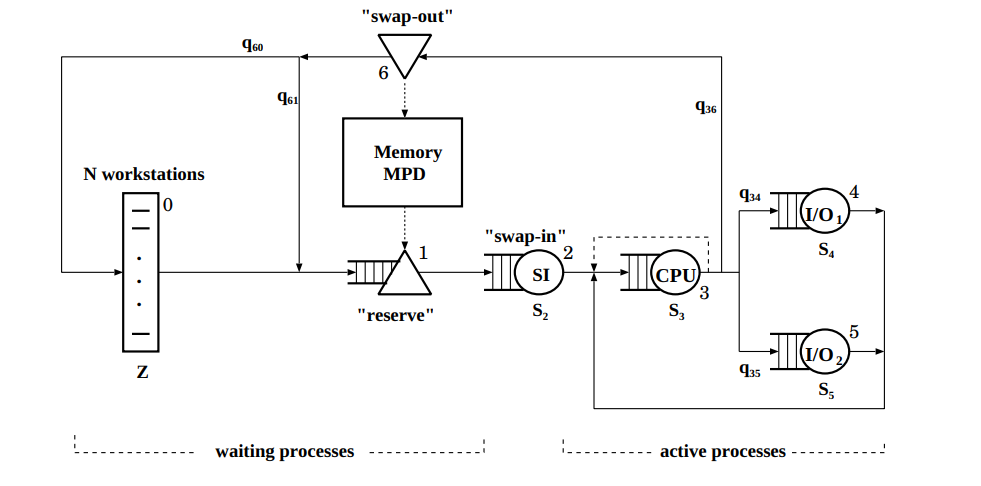
\includegraphics[width=0.8\textwidth]{Images/model.png}
			
			\vfill
			
			
			
			\vspace{0.8cm}
			
			
			
			\Large
			
			
			
			
		\end{center}
		\Large
		\begin{tabbing}
			\hspace*{1em}\= \hspace*{8em} \= \kill % set the tabbings
			\> Name:\>  \textbf{Matteo Ielacqua} \\
			\> ID:\>  \textbf{839241} \\
		\end{tabbing}
		
	\end{titlepage}
	
	
	
	\section{Description of the simulator}
    In this section a brief analysis of the code and other technical aspect of the simulator will be discussed.
    \subsection{Events}
    The simulator is designed to manage a range of events within this system, with a particular focus on two crucial types: the arrival of a client and the departure. Each event type has a distinct impact on the simulator's state, influenced by the specific target under consideration. 
    \begin{itemize}
        \item Departure from the delay station: a departure from the delay station will cause an arrival at the swap-in station.
        \item Arrival to the delay station: an arrival will trigger a departure with a certain delay, that is a Random Variable with a negative exponential distribution of 5000 ms .
        \item Arrival at the Reserve station: if the counter of the process allocated in the system is less than the setted MPD. Then the an arrival event is immediately scheduled for the swap in. Otherwise the information are stored in a queue for later use at the next arrival.
        \item Arrival at the swap in station: an arrival to this station will trigger a departure with a delay, equal to a RV with negative exponential distribution of 210 ms. If at the arrival the station is `occupied' by another client that is waiting it's departure, then the client will be served later with an FCFS policy.
        \item Departure from the swap in station: a departure from the swap in will trigger an immediate arrival to the CPU 
        \item Arrival to the CPU: An arrival to the cpu can be of 2 types, 1) the arrival of a new process has happened, so it is either stored in the ready queue if an another process is under execution or it's executed immediately. In this process a service time with an hyper exponential distribution is assigned to the service. 2) a process that was enqueued in the ready queue is rescheduled for execution , no event under process is expected under this assumption because this type of arrival is accepted only if a departure has appened in the CPU. The exeuction of a process is simulated by scheduling a departure with a delay equal to the time slice of the cpu and subtracting the remaining service time of the process with that time slice.
        \item Departure from the CPU: this event can happen in different conditions which will lead to 2 different behaviour: 1) the process has a remaining service time > 0, so it will be memorized in the ready queue for later use, at this point a new process is Dequeued from the ready queue and scheduled for execution (arrival to the CPU), the actual event under process is resetted. 2) the remaining service time of the process is 0, so an arrival is triggered to the IO1, IO2 or the Swap out with a certain routing probability. A new process is extracted from the ready queue if it is available.
        \item Arrival to IO1/IO2: in both cases an arrival will trigger a departure from the relative station that is an RV with negative exponential distribution.
        \item Departure from IO1/IO2: in both cases this will result in an immediate arrival event to the CPU. 
        \item Arrival to swap out: this event will trigger an immediate departure for the swap out 
        \item Departure from swap out: this event will trigger an immediate arrival to the delay station with p 0.4 or an immediate arrival to the reserve station with p 0.6. In any case this event will decrement by 1 the counter of allocated process in the reserve station.
    \end{itemize}

    \subsection{Choice of the regeneration point}
    Since the technique of the tagged customer is used a particular attention must be put in the event that will raise a possible regeneration point. Considering that the target is to : estimate the active time of the client after a departure from the swap in and before it enter the swap out, it naturally follow that the set of station ("CPU","IO1","IO2") can be considered as an independent subsystem. Then a suitable option is to consider the entrance of the tagged customer as a regeneration point event. In order to be relevant a regeneration point must come with a proper description of the state of the system, in this case considering that the CPU is the unique station that has not a negative exponential distribution of the service times, this one must be empty in order to collect some valid data. IO2 is the bottleneck station, so is expected that an high value of client shall be present in this station, since the reserve station is limiting the number of maximum process present in this subsystem a good number of pilot simulation was performed, and showed that when the tagged customer enter the system the IO2 contains 7 clients , in the whole station, with a good probability. Same reasoning was applied for the IO1, that lead to choose a value of 2 clients in the station. The conditions are then: Tagged customer at the entrance of the subsystem, 7 clients at the IO2, 2 clients at the IO1 and 0 clients at the CPU, the others are in the swap in, reserve station or delay station.
    \section{First validation step}
    \subsection{Bottleneck analysis}
    In order to start the analysis , let's show here the simplified model 
    used to conduct the validation.
    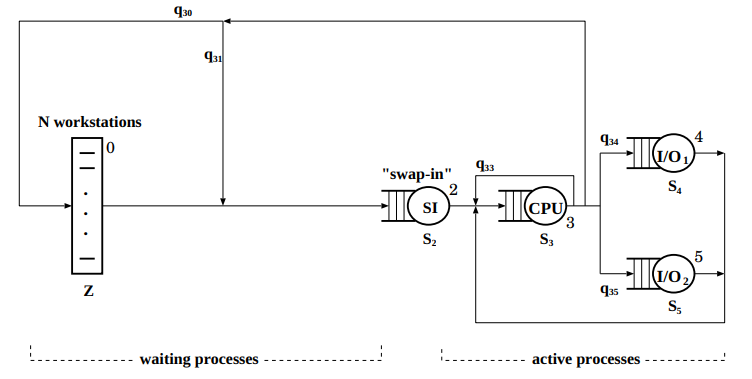
\includegraphics[width=0.8\textwidth]{Images/simplified_model.png}
    \\And summarize some data:
    \begin{displaymath}
        \begin{aligned}
        S_2 = 210ms && S_3= 2.7ms && S_4 = 40ms && S_5=180ms\\
        q_{3,0}= 0.4&& q_{3,1}=0.6 && q_{3,3} = 0.9 && q_{3,4}= 0.065\\
        && q_{3.5}= 0.025 && q_{3,6}=0.01 && 
        \end{aligned}
    \end{displaymath}
    Based on this data, it becomes evident that the provided approximation is plausible. Given a process with a 0.9 probability of returning with a mean service time of 2.7, and considering our original model where clients exhibit a mean service time of 27 ms and a fixed CPU slice time of 2.7 ms, we anticipate that a customer will be rescheduled in the CPU nearly nine additional times following the initial scheduling. \\

    From the previous data we can extract this matrix 
    \begin{displaymath}
        \begin{bmatrix}
            0 && 1 && 0 && 0 && 0 \\
            0 && 0 && 1 && 0 && 0 \\
            0.004 && 0.006 && 0.9 && 0.065 && 0.025 \\
            0 && 0 && 1 && 0 && 0 \\
            0 && 0 && 1 && 0 && 0 \\
        \end{bmatrix}
    \end{displaymath}

    From which we can extract the following system of equations 
    \begin{displaymath}
        \begin{cases}
            V_0=0.004V_3\\
            V_2=V_0+0.006V_3\\
            V_3=V_2+0.9V_3+V_4+V_5\\
            V_4=0.065V_3\\
            V_5= 0.025V_3
        \end{cases}
    \end{displaymath}
    with the additional equation $V_0=1$. Resolving this system lead to the computation 
    all $V_i$ 
    \begin{displaymath}
        \begin{cases}
            V_0=1 \\
            V_3=250\\
            V_2=2.5\\
            V_4=16.25\\
            V_5=6.25
        \end{cases}
    \end{displaymath}

    From this computes $V_i$ is possible to detect which of the station is the bottleneck of the system
    by considering that $VbS_b= \max_i\{V_iS_i\}$, so let's compute all $V_iS_i$ and find 
    the greater one. 

    \begin{displaymath}
        \begin{aligned}
            V_2S_2= 525ms && V_3S_3=675ms && V_4S_4=650ms && V_5S_5= 1125ms
        \end{aligned}
    \end{displaymath}
    from this calculation we can say that $V_bS_b=V_5S_5=1125ms$ and so , station 5 (IO2) is 
    our bottleneck. Let's extract some additional information, as the total cycle time when $N=1$ ,i.e Y(1) 
    \begin{displaymath}
        D=\sum_{i=1}^{N}D_i=\sum_{i=1}^{N}V_iS_i + V_0S_0=7975ms
    \end{displaymath}
    Thus we can also calculate the saturation point $N^*$ of this system, after which we can expect
    the total response time will increase. 
    \begin{displaymath}
        N^*=\frac{Y(1)}{V_bS_b}=\frac{D}{V_bS_b}=\frac{7975ms}{1125ms}=7.08
    \end{displaymath}
    \subsection{MVA analysis}
    Starting from the previous matrix is possible to compute various measures using the MVA algorithm for Load Indipendent and Delay stations. In order to compute the visits vector is possible to use the power matrix method.
    \begin{lstlisting}[language=C++]
        
    std::vector<double> 
    powerMatrixMethod(Matrix<double> dtmc, int iterations)
    {
        auto old = dtmc;
        auto res = old;
        for(int i = 0; i < iterations; i++){
            res = old*old;
            old = res;
        }

        std::vector<double> result{};
        for(int i = 0; i < res.Rows(); i++)
            result.push_back(res(i,i));
        return result;
    }
    \end{lstlisting}
    That requires only to multiply the transition matrix for an arbitrary number of iterations, then pick the elements on the diagonal, that are the probability mass flowing in to the i-th station. Let the previously obtained vector be $D$, at this point the visits can be computed with this simple formula $V_i=D_i*\frac{1}{D_0} \ \ \ i=1 \dots N$. In c++ this translate to:
    \begin{lstlisting}[language=C++]
        // compute the visits vector with 
        // 10000 iteration of power matrix method
        std::vector<double> visits = powerMatrixMethod(q, 10000);
        for (int i = 1; i < visits.size(); i++)
        {
            visits[i] = visits[i] * (1 / visits[0]);
        }
    \end{lstlisting}
    At this point is possible to apply the MVA algorithm, that result in subsequent values.
    \\
    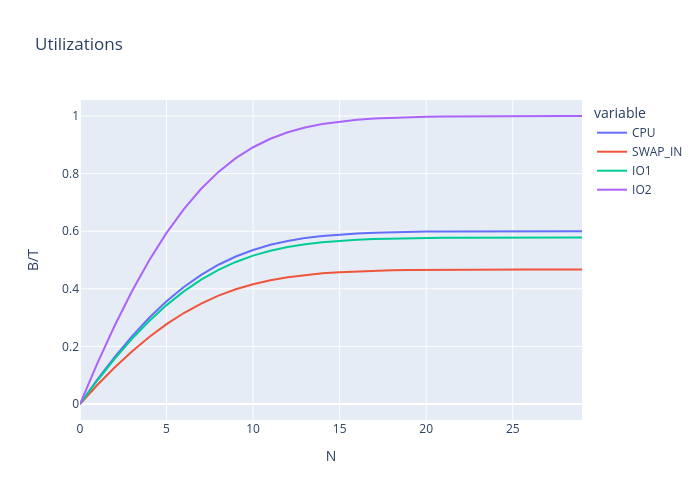
\includegraphics[width=0.9\textwidth]{Images/Utilizations.png}\\
    From the utilization functions we can conclude that the bottleneck station is IO2, as confirmed by the bottleneck analysis. Also becomes evident that after the saturation point ($N \approx7$) the growth of utilization tend to diminish despite the linear increase of N.
    \\
    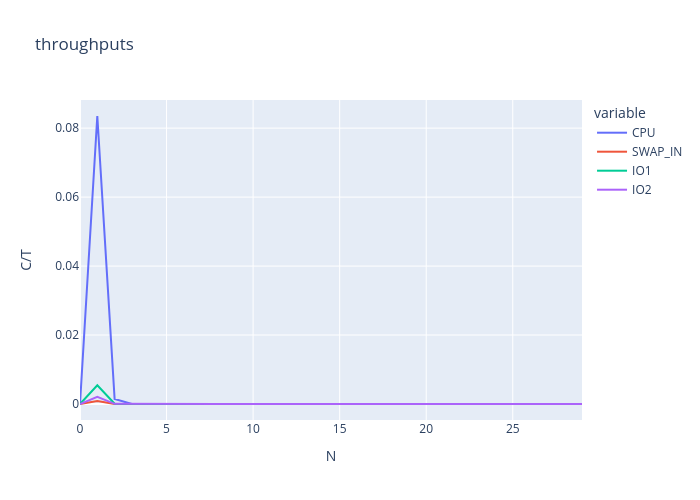
\includegraphics[width=0.9\textwidth]{Images/throughputs.png}
    \\
    Also from the throughputs the same statement can be reached, but with a particular observation on the CPU, that gradually stop the increasing of the throughput as N becomes larger then 7. This phenomena is similar to a very well known problem in the operative system ecosystem: thrashing. In this case the thrashing is caused by the massive use of the IO2 from the processes involved, so the throughput of the CPU will not decrease but remain steady as it will depend entirely on the process capacity of the IO2. 
    \\
    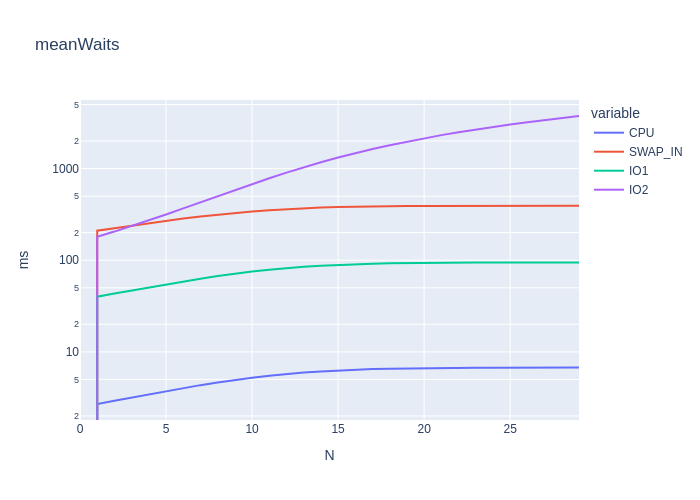
\includegraphics[width=0.9\textwidth]{Images/meanWaits.png}
    \\
    Mean waits also confirm that the bottleneck station is the IO2, since all other don't increase their mean wait time at the increase of N.
    \\
    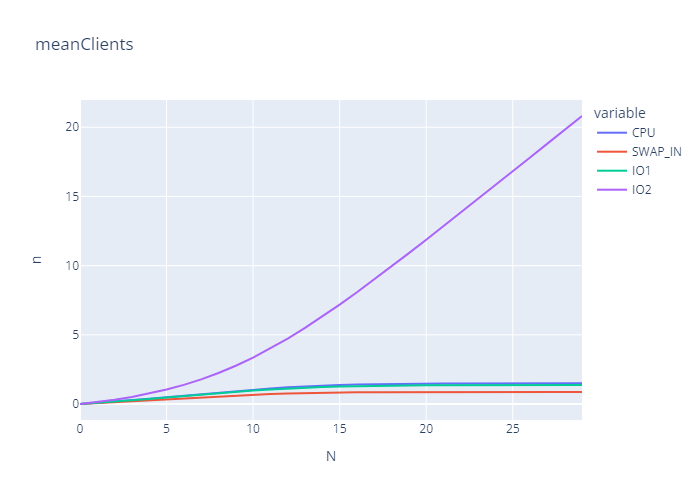
\includegraphics[width=0.9\textwidth]{Images/meanClients.png}
    \\
    In this graph the tendency of the IO2 station to be a bottleneck is much visible, since the customers tend to increase the queue size of the IO2 at the increase of N.
    \\
    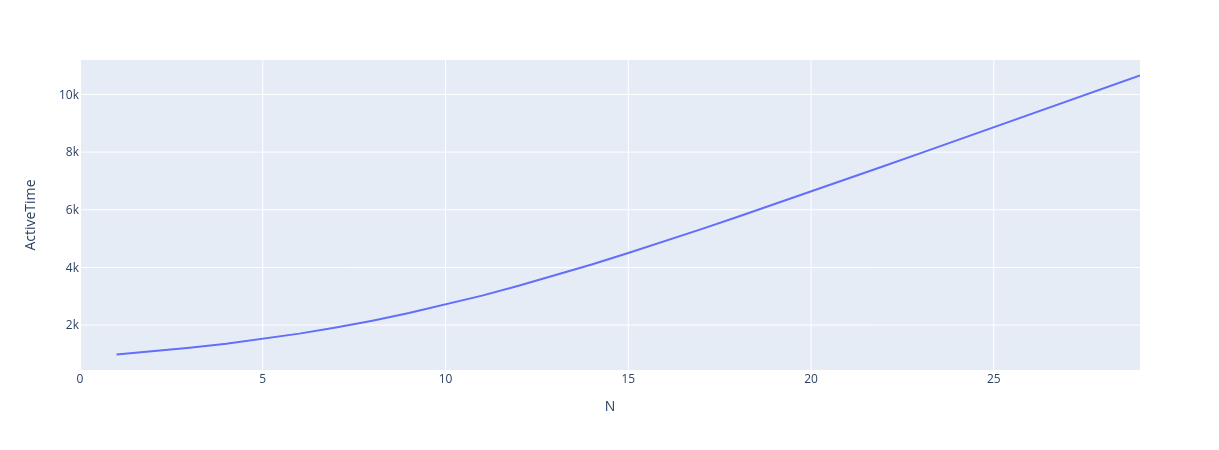
\includegraphics[width=0.9\textwidth]{Images/ActiveTimes.png}
    \\
    Considering the subsystem composed by IO1,IO2 and CPU we can estimate then the active time of a client with little effort, resorting to little's formula 
    $$
    \bar{w}= \frac{\bar{n}}{\lambda}
    $$
    since all the clients are coming from the swap in, then it's throughput becomes the arrival rate of the formula. The data show that with N=20 a value of 6630 should be expected.
    \section{Simulation Results}

    \subsection{The simplified model used for MVA}
    The first scenario is the case where we have a condition in which $MPD>>N$ , burst time = time slice and there is a routing probability of 0.9 that the departured client will return to CPU. In this case the limitation imposed by the reserve station is not considered, hence the measure collected by the simulator should be similar to the ones calculated by MVA. In this case with a seed of 123456789 the following measure are obtained 
    \begin{center}
        \begin{tabular}{ |c|c|c|c|c}
            Station & Mean N & Mean W & Expected W & Expected N \\
            CPU & (LB:1.42592, LH:1.48144) & (6.490457,6.65112) & 6.65302 & 1.47487
            
        \end{tabular}        
    \end{center}


    \subsection{Default Scenario}
    The default scenario (case 1) has the following characteristics:
    \begin{itemize}
        \item Time slice: 2.7ms 
        \item Burst with hyper exponential distribution with : $\alpha$ = 0.95 and $\beta$ = 0.05, $u_1=10 ms$ and $u_2=350 ms$.
    \end{itemize}
    
    \section{Simulator description}
    \subsection{Brief description of the implementation}
    The simulator is substantially a shell. The program loads at the beginning the skeleton of the simulator composed by an OS object. Such object hold the description of the model composed by a Round Robin station (class CPU), a delay station (class DelayStation) and all the other First Come First Served (class FCFSStation). The OS Object inherit from scheduler that hold the main event queue and manage all the operations inside the simulator. OS also inherit from the class Simulator, that substantially contains all the functions that are need to pilot the execution, such as dequeue an event , route it to the right station and so on. The environment of simulation is divided in 3 abstraction layers: 
    \begin{itemize}
        \item class SimulationEnvironment
        \item class SimulationResult 
        \item class SimulationShell
    \end{itemize}
    \subsubsection{SimulationEnvironment}
    This class hold the setup functions for the base system and each scenario. Scenarios are a short way to describe the regeneration point for that scenario and the parameter for the simulation (for example the cpu slice time). In all the four case described the regeneration point is the same, but the parameter (especially for the CPU) are different. This class also contains the SimulationResult data strucuture, which holds all the accumulators.
    \subsubsection{SimulationResult}
    SimulationResult class hold all the accumulator used to display the result of the simulator, it contains various function for register 2 particular measure of all the station involved: mean waits and mean clients. At the end of each regeneration cycle the measure are extracted from the OS class.
    \subsubsection{SimulationShell}
    this class hold all the functions need to make the program interactive, in the section Available commands various input can be used to manipulate the simulator. The principal facilities of this class let the user to create a Command structure, which pair a sequence of character to an action.
    \subsection{Available commands}  
    \begin{itemize}
        \item help: display an help with all the commands 
        \item verbosity <list|sourceName> [int] : let the user to select a verbosity for a source, the sources can be listed with list. Note that all the station have verbosity 1 in order to not display the actual processing of the events.
        \item start: manually start the simulator
        \item stop: manually stop the simulator 
        \item init: initialize the system , it is needed after each call to scenario.
        \item clock: display the actual clock of the simulation.
        \item ne [int]: process a certain number of events 
        \item seed: set the seed for the simulator 
        \item hreset: reset completely the state of the simulator 
        \item exit: quit the program 
        \item regstats: display the statistics on hit and call of regeneration point , each hit correspond to an event that call the regeneration point, each call correspond to the regeneration point being satisfied.
        \item env: Display the environment variables (SystemParameters) that describe the scenario used for the simulator (MPD, slice ecc\dots)
        \item lstats: Display the actual status of the stations , B=busy time, O= observation time, A=arrivals,C=completions,N: sysclients, W:meanWaits (sample mean), MAXN: max sysclients observed, AN: area of N (sysclients*interval), AS:area of S ((sysclients-1)*interval).
        \item lqueue <name>: Display the actual status of all the queues
        \item scenario <list|scenarioname>: set the scenario for the simulation. A brief description of the available scenario is available in the section Scenarios.
        \item nr <numCycles:0+|untilPrecisionReached:-1> <showMeasure:1|0>: compute the n regeneration cycle or stop when the requested precision (0.05) is reached (using -1 as argument). The second argument ask to display or not the measure after each regeneration cycle (0 false, 1 true).
        \item na <CPU|IO1|IO2|SWAP\_IN>: Execute the simulation until an arrival is detected to the station listed.
        \item nd <CPU|IO1|IO2|SWAP\_IN>: Execute the simulation until a departure is detected to the station listed.
        \item nn <seed:int> <numSimulations:int> <showMeasure:1|0> : Execute a fixed number of simulation reaching the precision requested every time, at the end of each simulation it will compare with MVA result and tell if the confidence interval has the true mean or not.
        \item ltgtstats: print the cycle time catched by the tagged customer
        \item lmeasures: print all the collected measure
        \item reset\_measures: manually reset all the accumulators
        
    \end{itemize}
    \end{document}